\chapter{Inleiding}
\section{Compilers}
Voorbeelden van functies die een statische compiler moet bevatten:
	\begin{itemize}
		\item Broncode omzetten in uitvoerbare fouten.
		\item Syntaxfouten moeten herkent worden.
	\end{itemize}

\section{Basiswerking compilers}
\begin{figure}[h]
	\centering
	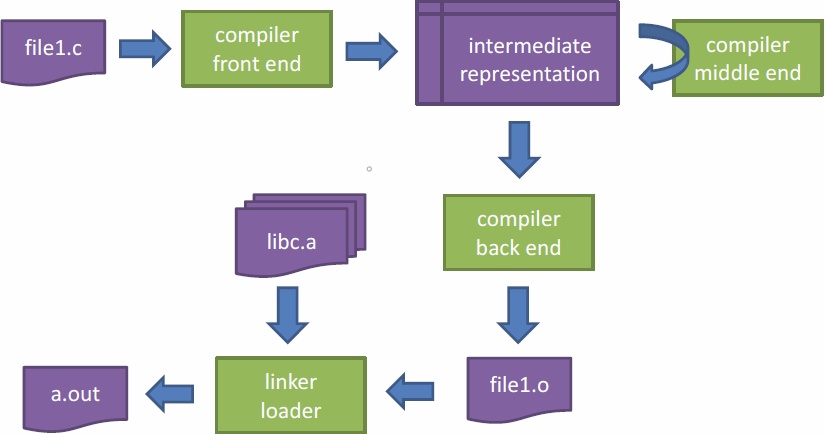
\includegraphics[width=0.5\textwidth]{basiswerking_compilers}
	\caption{De basiswerking van een compiler.} 
	\label{fig:basiswerking_compilers}
\end{figure}
Op figuur \ref{fig:basiswerking_compilers} is de vereenvoudigde basiswerking van een compiler te zien. Een \textbf{C} bestand wordt eerst door de \uline{compiler front end} gestuurd, die het bestand zal omvormen tot een intermediaire representatie. Deze representatie wordt dan door de \uline{compiler back end} gestuurd om zo assembly of objectcode te genereren. De \uline{linker loader} zal deze objectcode samenvoegen met eventuele andere libraries om zo een uitvoerbaar programma te hebben. 

\QA{Waarom wordt de front end en back end opgesplitst?}
{Op die manier is de compiler modulair: Enerzijds moet bij een andere programmeertaal enkel de front end aangepast worden en anderzijds moet bij het wijzigen van de architectuur (de onderliggende processor) enkel de back end aangepast worden.}


\section{Abstract Syntax Tree}
De eerste stap van elke compiler is het omvormen van de broncode naar een \textbf{Abstract Syntax Tree (AST)}. Veronderstel volgende code, en de daarbijhorende AST die te zien zijn op figuur \ref{fig:abstract_syntax_tree}. Elke knoop van een AST stelt een bepaalde geldige operatie voor, die onafhankelijk is van de gekozen programmeertaal.
\begin{figure}[h]
	\centering
	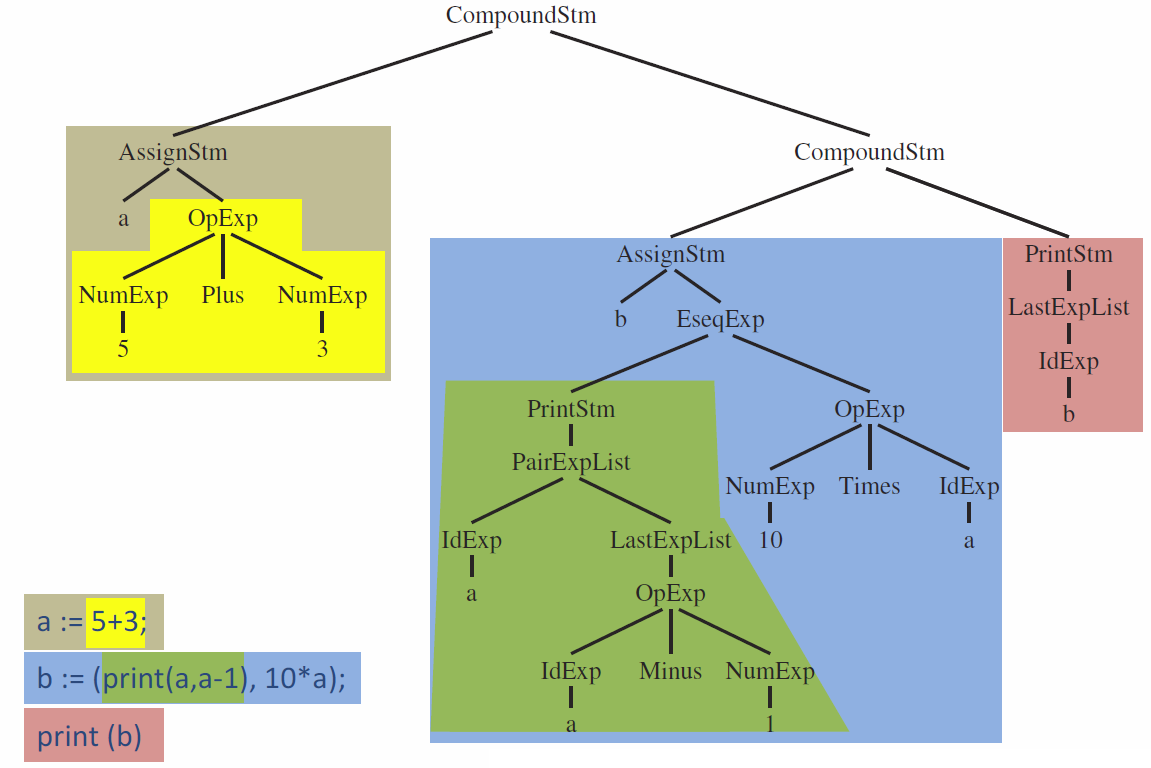
\includegraphics[width=0.8\textwidth]{abstract_syntax_tree}
	\caption{De boomvoorstelling van een eenvoudig, lusloos programma. De gekleurde deelbomen komen overeen met de gekleurde segmenten in de code zelf. Als toekenningsoperator wordt er gekozen voor $:=$ dat vanaf nu als één geheel moet beschouwd worden.}
	\label{fig:abstract_syntax_tree}
\end{figure}

\subsection{Generatieve grammatica's}
Om een AST op te stellen moet de notie van tokens ingevoerd worden. Een token is eenvoudig gezien een bepaald symbool dat een betekenis heeft. De tokens van de code uit figuur \ref{fig:abstract_syntax_tree} zijn te zien in tabel \ref{table:tokens}
\begin{table}[h]
	\centering
	\begin{tabular}{l | l | l}
		symbolen(ascii) & token & waarde \\
		\hline
		a & id & string a \\
		:= & := & \\
		5 & num & integer 5 \\
		+ & + & \\
		3 & num & integer 3 \\
		; & ; & \\
		b & id & string b \\
		( & ( & \\
		print & print & \\
		- & - & \\
		* & * & \\
		  & whitespace & \\
	\end{tabular}
	\caption{De tokens die voorkomen uit het programma van figuur \ref{fig:abstract_syntax_tree}}
	\label{table:tokens}
\end{table}
Uit de theorie van de generatieve grammatica's weten we dat er zowel terminale als niet-terminale tokens bestaan:
\begin{itemize}
	\item \textbf{Terminale tokens} zijn symbolen die een blad voorstellen in de AST. Deze tokens hebben als eigenschap dat ze geen verdere tokens kunnen genereren en vormen dan ook het alfabet van het programma.
	\item \textbf{Niet-terminale tokens}, kortweg niet-terminalen genoemd, zijn de regels die de taal definiëren en zijn de niet-bladeren van de AST. Niet-terminalen hebben als eigenschap dat ze letters van het alfabet kunnen genereren.
\end{itemize}
Op figuur \ref{fig:contextvrije_grammatica} zijn een aantal terminalen en niet-terminalen te zien. De niet-terminale token \textit{CompoundStm} bestaat bijvoorbeeld uit twee \textit{Stm} tokens, gescheiden door een punt komma. Deze twee \textit{Stm} tokens kunnen in deze vereenvoudigde programmeertaal enkel een \textit{AssignStm} of \textit{PrintStm} zijn. Bij \textit{AssignStm} wordt er een terminale token verwacht in de vorm van een variabele identifier, gevolgd door de toekenningsoperator en een \textit{Exp} token. Enkel deze \textit{Exp} kan nog vier vormen aanneemen: \textit{IdExp}, \textit{NumExp}, enz...

\begin{figure}[h]
	\definecolor{cvred}{RGB}{215,149,146}
	\definecolor{cvblue}{RGB}{145,202,219}
	\centering
	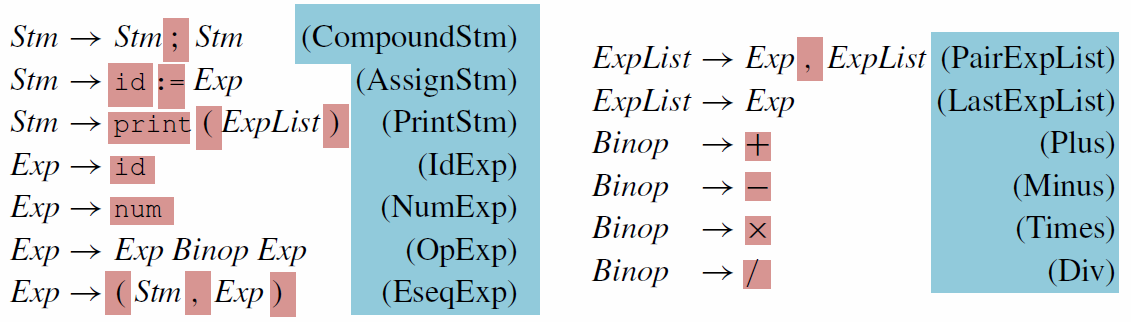
\includegraphics[width=0.8\textwidth]{contextvrije_grammatica}
	\caption{De rood omkaderde symbolen zijn {\color{cvred} terminalen} terwijl de blauw omkaderde {\color{cvblue}niet-terminalen} zijn.} 
	\label{fig:contextvrije_grammatica}
\end{figure}

Dit wordt uitgewerkt op figuur \ref{fig:abstract_syntax_tree} voor de eerste toekenningsoperatie op figuur \ref{fig:contextvrije_grammatica_voorbeeld}.
\begin{figure}[h]
	\centering
	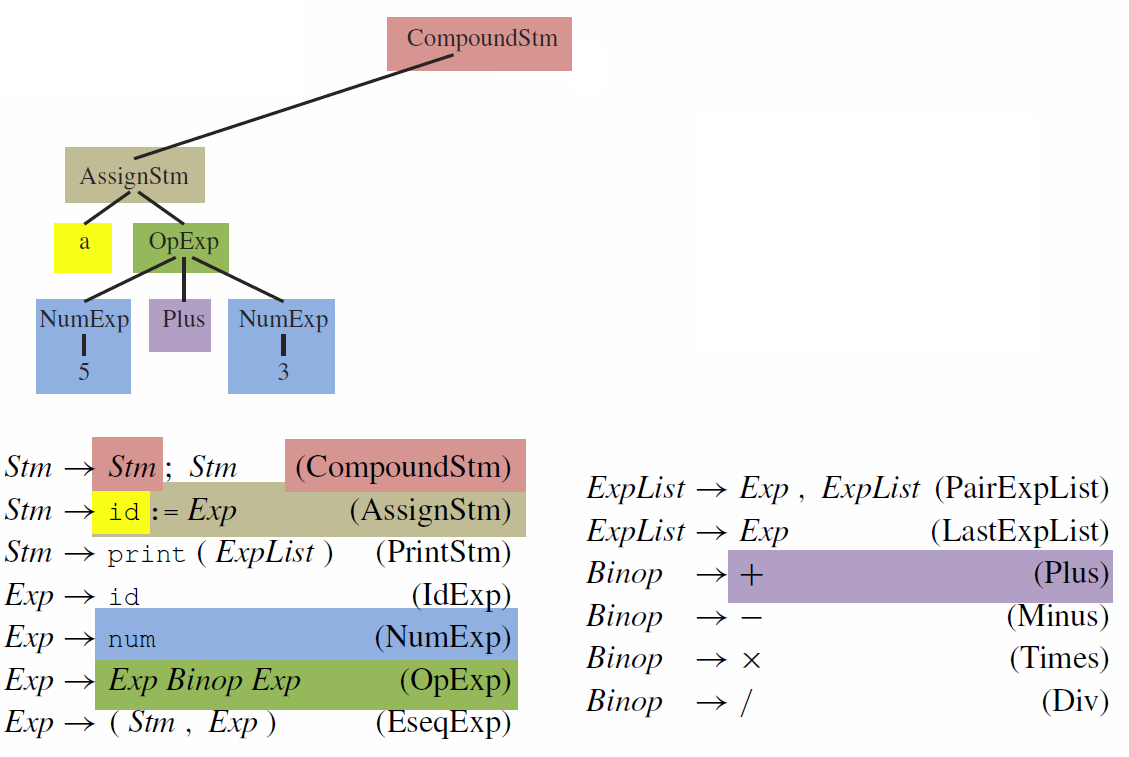
\includegraphics[width=0.8\textwidth]{contextvrije_grammatica_voorbeeld}
	\caption{Illustratie van contextvrije grammatica op de eerste toekenningsoperatie uit figuur \ref{fig:abstract_syntax_tree}.} 
	\label{fig:contextvrije_grammatica_voorbeeld}
\end{figure}

\subsection{Opbouw AST}
Een AST kan nu \textbf{bottom-up} opgemaakt worden door volgende procedure uit te voeren:
\begin{enumerate}
	\item Voor elke mogelijke knoop moet er een struct gemaakt worden zoals bijvoorbeeld:
	
	$$\texttt{A\_stm\_} \qquad \texttt{A\_exp\_} \qquad \texttt{A\_expList\_}$$
	
	\item Elke struct moet bestaan uit
	\begin{itemize}
		\item een enum voor het precieze token te bepalen,
		\item een union voor de verschillende combinaties van tokens in het rechter lid en,
		\item pointers naar kindknopen.
	\end{itemize}
	Dit wordt geïllustreerd in code \ref{lst:code}.
	\begin{lstlisting}[caption={Voorbeeld van een struct voor een AST.},label={lst:vb_struct_AST}, captionpos=b]
typedef char * string;
typedef struct A_stm_ * A_stm;
typedef struct A_exp_ * A_exp;
typedef struct A_expList_ * A_expList;

struct A_stm_ {
	enum {A_compoundStm, A_assignStm, A_printStm} kind;
	union {
		struct {A_stm stm1, stm2;} compound;
		struct {string id; A_exp exp;} assign;
		struct {A_expList exps;} print;
	} u;
};
	\end{lstlisting}
	\item In de constructor worden de knopen aangemaakt, zoals te zien in code \ref{lst:vb_constructor_AST}.
	\begin{lstlisting}[caption={Voorbeeld van een constructor voor een AST.},label={lst:vb_constructor_AST}, captionpos=b]
A_stm A_CompoundStm(A_stm stm1, A_stm stm2){
	A_stm s = malloc(sizeof(*s));
	s->kind = A_compoundStm;
	s->u.compound.stm1 = stm1;
	s->u.compound.stm2 = stm2;
	return s;
}
	\end{lstlisting}
	
Op deze manier zou de boom uit figuur \ref{fig:abstract_syntax_tree} hardgecodeerd kunnen worden, wat natuurlijk geen goede manier is. Het is de taak van een \uline{lexer} en \uline{parser} om de constructie van een AST te automatiseren, \todo{refereren naar volgende hoofdstukken}

\subsection{Interpreter}
\todo{Stukje over interpreter}

\end{enumerate}


